%\title{LaTeX Portrait Poster Template}
%%%%%%%%%%%%%%%%%%%%%%%%%%%%%%%%%%%%%%%%%
% a0poster Portrait Poster
% LaTeX Template
% Version 1.0 (22/06/13)
%
% The a0poster class was created by:
% Gerlinde Kettl and Matthias Weiser (tex@kettl.de)
% 
% This template has been downloaded from:
% http://www.LaTeXTemplates.com
%
% License:
% CC BY-NC-SA 3.0 (http://creativecommons.org/licenses/by-nc-sa/3.0/)
%
%%%%%%%%%%%%%%%%%%%%%%%%%%%%%%%%%%%%%%%%%

%----------------------------------------------------------------------------------------
%	PACKAGES AND OTHER DOCUMENT CONFIGURATIONS
%----------------------------------------------------------------------------------------

\documentclass[a0,portrait]{a0poster}

\usepackage{lineno}
\usepackage{array}
\usepackage{lscape}
\usepackage{graphicx}
\usepackage{subcaption}
\usepackage{float}
\usepackage{multicol} % This is so we can have multiple columns of text side-by-side
\usepackage{amsmath}
\columnsep=100pt % This is the amount of white space between the columns in the poster
\columnseprule=3pt % This is the thickness of the black line between the columns in the poster

\usepackage[svgnames]{xcolor} % Specify colors by their 'svgnames', for a full list of all colors available see here: http://www.latextemplates.com/svgnames-colors

\usepackage{times} % Use the times font
%\usepackage{palatino} % Uncomment to use the Palatino font

\usepackage{graphicx} % Required for including images
\graphicspath{{figures/}} % Location of the graphics files
\usepackage{booktabs} % Top and bottom rules for table
\usepackage[font=small,labelfont=bf]{caption} % Required for specifying captions to tables and figures
\usepackage{amsfonts, amsmath, amsthm, amssymb} % For math fonts, symbols and environments
\usepackage{wrapfig} % Allows wrapping text around tables and figures

\newcommand{\bbbar}{$b\bar{b}$}
\newcommand{\afb}{$A_{FB}^b$}
\newcommand{\sm}{Standard Model}
\newcommand{\bsm}{Beyond Standard Model}
\newcommand{\mF}{\mathcal{F}^I}

\begin{document}

%----------------------------------------------------------------------------------------
%	POSTER HEADER 
%----------------------------------------------------------------------------------------


\begin{minipage}[b]{1.\linewidth}
\veryHuge \color{NavyBlue} \textbf{Studies of $e^+e^-\to b\bar{b}$ channel at the International Linear Collider} \color{Black} % Title
 % Subtitle
\end{minipage}
\begin{minipage}[b]{0.5\linewidth}
\Huge\textit{Final word on LEP \afb\ anomaly}\\[1cm]
\huge \textbf{\underline{BILOKIN S.}, P\"OSCHL R., RICHARD F.}\\[0.5cm] % Author(s)
\huge Laboratoire de l'Acceler\'ateur Lin\'eare\\[0.4cm] % University/organization
\Large \texttt{bilokin@lal.in2p3.fr}\\
\end{minipage}
%
\begin{minipage}[b]{0.5\linewidth}

\includegraphics[height=9cm]{figures/LAL.jpg}

\includegraphics[height=9cm]{figures/UPSUD.jpg}

\includegraphics[height=9cm]{figures/logo-ild.png}\\
\end{minipage}

\vspace{1cm} % A bit of extra whitespace between the header and poster content

%----------------------------------------------------------------------------------------

\begin{multicols}{2} % This is how many columns your poster will be broken into, a portrait poster is generally split into 2 columns

%----------------------------------------------------------------------------------------
%	ABSTRACT
%----------------------------------------------------------------------------------------

\color{Navy} % Navy color for the abstract

\begin{abstract}

This poster presents studies for the International Linear Collider (ILC), a linear electron-positron collider with a nominal center-of-mass energy from 250\,GeV to 500\,GeV.

The results of the detector study allow for an estimation of the ILC precision on the b-quark electroweak couplings and form factors. The ILC will be able to resolve the LEP anomaly in the \bbbar\ production process. The ILC precision on the right-handed $Z^0b\bar{b}$ coupling, a prime candidate for effects of new physics, is calculated to be at least 5 times better than the LEP experiments. 
\end{abstract}

%----------------------------------------------------------------------------------------
%	INTRODUCTION
%----------------------------------------------------------------------------------------

\color{SaddleBrown} % SaddleBrown color for the introduction

\section*{Introduction}

Aliquam non lacus dolor, \textit{a aliquam quam} \cite{Smith:2012qr}. Cum sociis natoque penatibus et magnis dis parturient montes, nascetur ridiculus mus. Nulla in nibh mauris. Donec vel ligula nisi, a lacinia arcu. Sed mi dui, malesuada vel consectetur et, egestas porta nisi. Sed eleifend pharetra dolor, et dapibus est vulputate eu. \textbf{Integer faucibus elementum felis vitae fringilla.} In hac habitasse platea dictumst. Duis tristique rutrum nisl, nec vulputate elit porta ut. Donec sodales sollicitudin turpis sed convallis. Etiam mauris ligula, blandit adipiscing condimentum eu, dapibus pellentesque risus.

\textit{Aliquam auctor}, metus id ultrices porta, risus enim cursus sapien, quis iaculis sapien tortor sed odio. Mauris ante orci, euismod vitae tincidunt eu, porta ut neque. Aenean sapien est, viverra vel lacinia nec, venenatis eu nulla. Maecenas ut nunc nibh, et tempus libero. Aenean vitae risus ante. Pellentesque condimentum dui. Etiam sagittis purus non tellus tempor volutpat. Donec et dui non massa tristique adipiscing.

%----------------------------------------------------------------------------------------
%	OBJECTIVES
%----------------------------------------------------------------------------------------

\color{DarkSlateGray} % DarkSlateGray color for the rest of the content

\section*{Main Objectives}

\begin{enumerate}
\item Lorem ipsum dolor sit amet, consectetur.
\item Nullam at mi nisl. Vestibulum est purus, ultricies cursus volutpat sit amet, vestibulum eu.
\item Praesent tortor libero, vulputate quis elementum a, iaculis.
\item Phasellus a quam mauris, non varius mauris. Fusce tristique, enim tempor varius porta, elit purus commodo velit, pretium mattis ligula nisl nec ante.
\item Ut adipiscing accumsan sapien, sit amet pretium.
\item Estibulum est purus, ultricies cursus volutpat
\item Nullam at mi nisl. Vestibulum est purus, ultricies cursus volutpat sit amet, vestibulum eu.
\item Praesent tortor libero, vulputate quis elementum a, iaculis.
\end{enumerate}

%----------------------------------------------------------------------------------------
%	MATERIALS AND METHODS
%----------------------------------------------------------------------------------------

%------------------------------------------------

\subsection*{Description of the heavy quark production}
%First, one needs to define the most convenient parametrization of coupling or form factors of interest, and then express the observable quantities in terms of defined form factors. 
Electroweak production of the fermion pairs proceeds through the $f\bar{f}X$ vertex, where $X$ represents neutral vector bosons, photon or $Z^0$ boson.  The current at the $f\bar{f}X$ vertex can be expressed via form factors $F$ as 
\begin{equation}
\Gamma^{f\bar{f}X}_\mu (k^2,q,\bar{q}) = ie\{ \gamma_\mu (F^X_{1V}(k^2) + \gamma^5 F^X_{1A}(k^2)) - \frac{\sigma_{\mu\nu}(q-\bar{q})^\nu}{2m_f}(iF^X_{2V}(k^2) + \gamma^5 F^X_{2A}(k^2)) \},
\end{equation}
where $k^2= (q+\bar{q})^2$ is the four momentum squared of the exchanged vector boson, $q$ and $\bar{q}$ are the four vectors of the fermion $f$ and antifermion $\bar{f}$ and $m_f$ is the fermion mass. Further, $\gamma_\mu$ and $\gamma_5$ are the Dirac matrices, and $\sigma_{\mu\nu} = i/2(\gamma_\mu\gamma_\nu - \gamma_\nu\gamma_\mu)$.

The \sm\ values of the form factors are the following:
\begin{equation}
F^{f\gamma}_{1V} = Q^{f}, \ F^{f\gamma}_{1A} = 0, \ F^{fZ}_{1V} = \frac{I^f - 2Q^f\sin^2\theta_W}{2\cos\theta_W\sin\theta_W}, \ F^{fZ}_{1A} = - \frac{I^f}{2\cos\theta_W\sin\theta_W},
\label{formula:SMformFactors_3}
\end{equation}
and all $F_2$ factor are zero. In the Eq.~\ref{formula:SMformFactors_3} $I^f$ is the weak isospin number, $I^t = 1/2$ for top and $I^b = -1/2$ for bottom quark and $Q^f$ is the electric charge, $Q^t = 2/3$ and $Q^b = -1/3$.

%The form factors are related to fermion couplings with left and right-handed helicity to $Z^0$ boson:
The following definition of the left-handed and right handed $Z^0b\bar{b}$ couplings is used throughout the thesis: 
\begin{equation}
%g_L^Z = (F_{1V}^Z - F_{1A}^Z), \  g_R^Z = F_{1V}^Z + F_{1A}^Z, 
g_L^Z = I^f - Q^f\sin^2\theta_W, \  g_R^Z = -Q^f\sin^2\theta_W, 
\label{formula:EWcouplings_3}
\end{equation}
%the same relations are applied to the corresponding photon couplings $g^\gamma_L$.
%At the tree level, the \sm\ differential cross for the production
%of a fermion $f$ pair in $e^+e^-\to f\bar{f}$ at center-of-mass energy $\sqrt[]{s}$ can be written as

In case of the polarized beams, the fermion form factors can be expressed in terms of the helicity of the initial electrons~\cite{bib:Schmidt}:
\begin{eqnarray}
\mathcal{F}^L_{ij} = - F^\gamma_{ij} +  \frac{-1/2 + \sin^2\theta_W}{\cos\theta_W\sin\theta_W}\frac{s}{s-M^2_Z+i\Gamma_ZM_Z}F^Z_{ij},\\
\mathcal{F}^R_{ij} = - F^\gamma_{ij} +  \frac{\sin^2\theta_W}{\cos\theta_W\sin\theta_W}\frac{s}{s-M^2_Z+i\Gamma_ZM_Z}F^Z_{ij}    
\label{formula:PolFF_3}
\end{eqnarray}

where $i=1,2$ and $j=V,A$, $M_Z$ and $\Gamma_Z$ are the $Z^0$ boson mass and width, respectively.

The key expression for the studies is the differential cross section of $f\bar{f}$ production for electron beam polarization $I=L,R$, expressed via the defined form factors:

\begin{multline}
 %\frac{\pi\alpha^2 N_c\beta}{s}
\label{formula:DiffSigma_3}
\frac{d\sigma^I}{d\cos\theta} = \frac{3}{4} \mathcal{A} N_c \beta[ (1+\cos^2\theta) [(\mF_{1V}+\mF_{2V})^2+(\beta \mF_{1A})^2] -\\-4 \cos\theta (\mF_{1V}+\mF_{2V})\beta \mF_{1A} + \sin^2\theta [\gamma ^{-2} (\mF_{1V} +\gamma^2 \mF_{2V})^2] ]
\end{multline}
where $\mathcal{A} = 4\pi\alpha^2/3s$ with $\alpha$ as the electromagnetic running coupling, $N_c$ is the number of quark colors, $\beta$ and $\gamma$ are the velocity and the Lorentz factor of the produced fermion, respectively. 

%----------------------------------------------------------------------------------------
%	RESULTS 
%----------------------------------------------------------------------------------------

\section*{Results}

Donec faucibus purus at tortor egestas eu fermentum dolor facilisis. Maecenas tempor dui eu neque fringilla rutrum. Mauris \emph{lobortis} nisl accumsan. Aenean vitae risus ante.

%
Phasellus imperdiet, tortor vitae congue bibendum, felis enim sagittis lorem, et volutpat ante orci sagittis mi. Morbi rutrum laoreet semper. Morbi accumsan enim nec tortor consectetur non commodo nisi sollicitudin. Proin sollicitudin. Pellentesque eget orci eros. Fusce ultricies, tellus et pellentesque fringilla, ante massa luctus libero, quis tristique purus urna nec nibh.

Nulla ut porttitor enim. Suspendisse venenatis dui eget eros gravida tempor. Mauris feugiat elit et augue placerat ultrices. Morbi accumsan enim nec tortor consectetur non commodo. Pellentesque condimentum dui. Etiam sagittis purus non tellus tempor volutpat. Donec et dui non massa tristique adipiscing. Quisque vestibulum eros eu. Phasellus imperdiet, tortor vitae congue bibendum, felis enim sagittis lorem, et volutpat ante orci sagittis mi. Morbi rutrum laoreet semper. Morbi accumsan enim nec tortor consectetur non commodo nisi sollicitudin.



\begin{center}\vspace{1cm}
	\label{fig:BAsymmetryFinal_3}
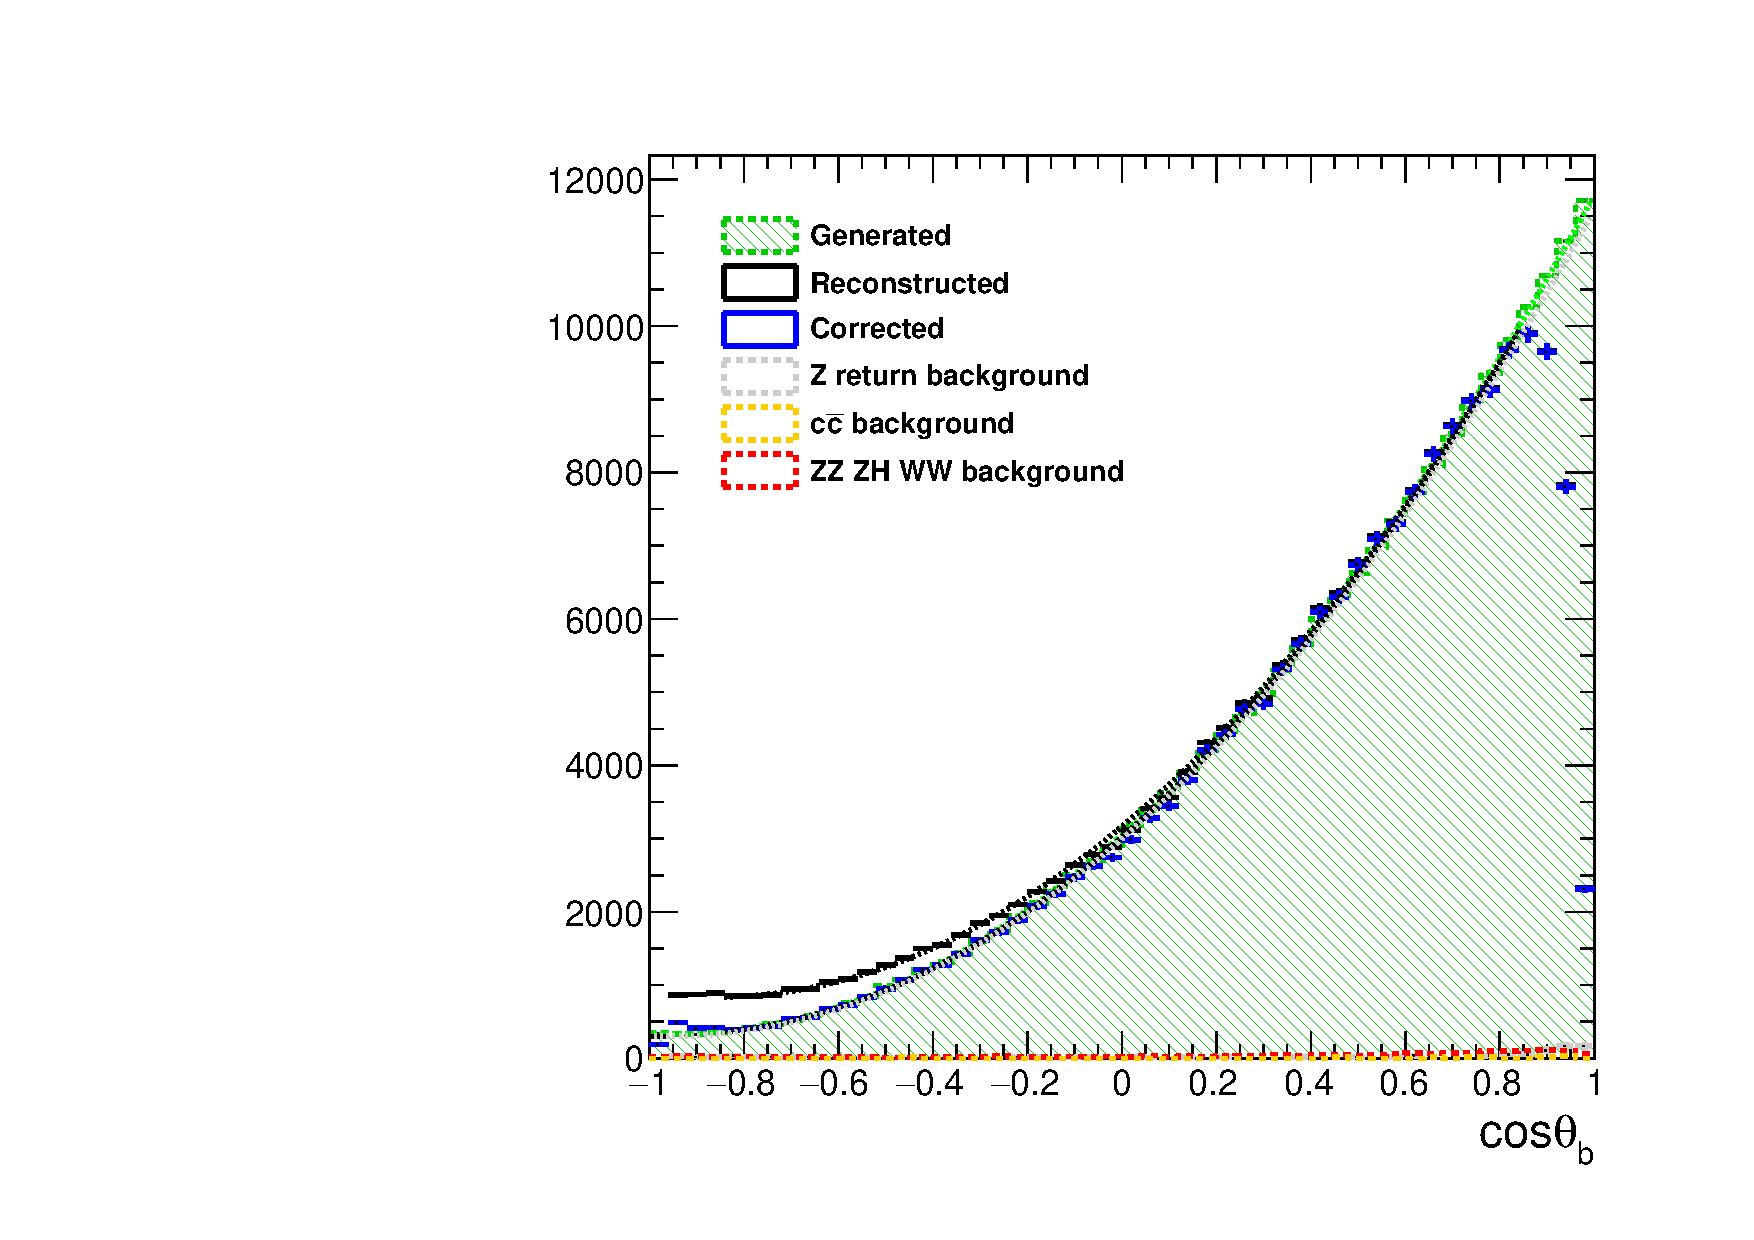
\includegraphics[width=0.49\linewidth]{../ILD/plots/basymmetry-final-left.pdf}
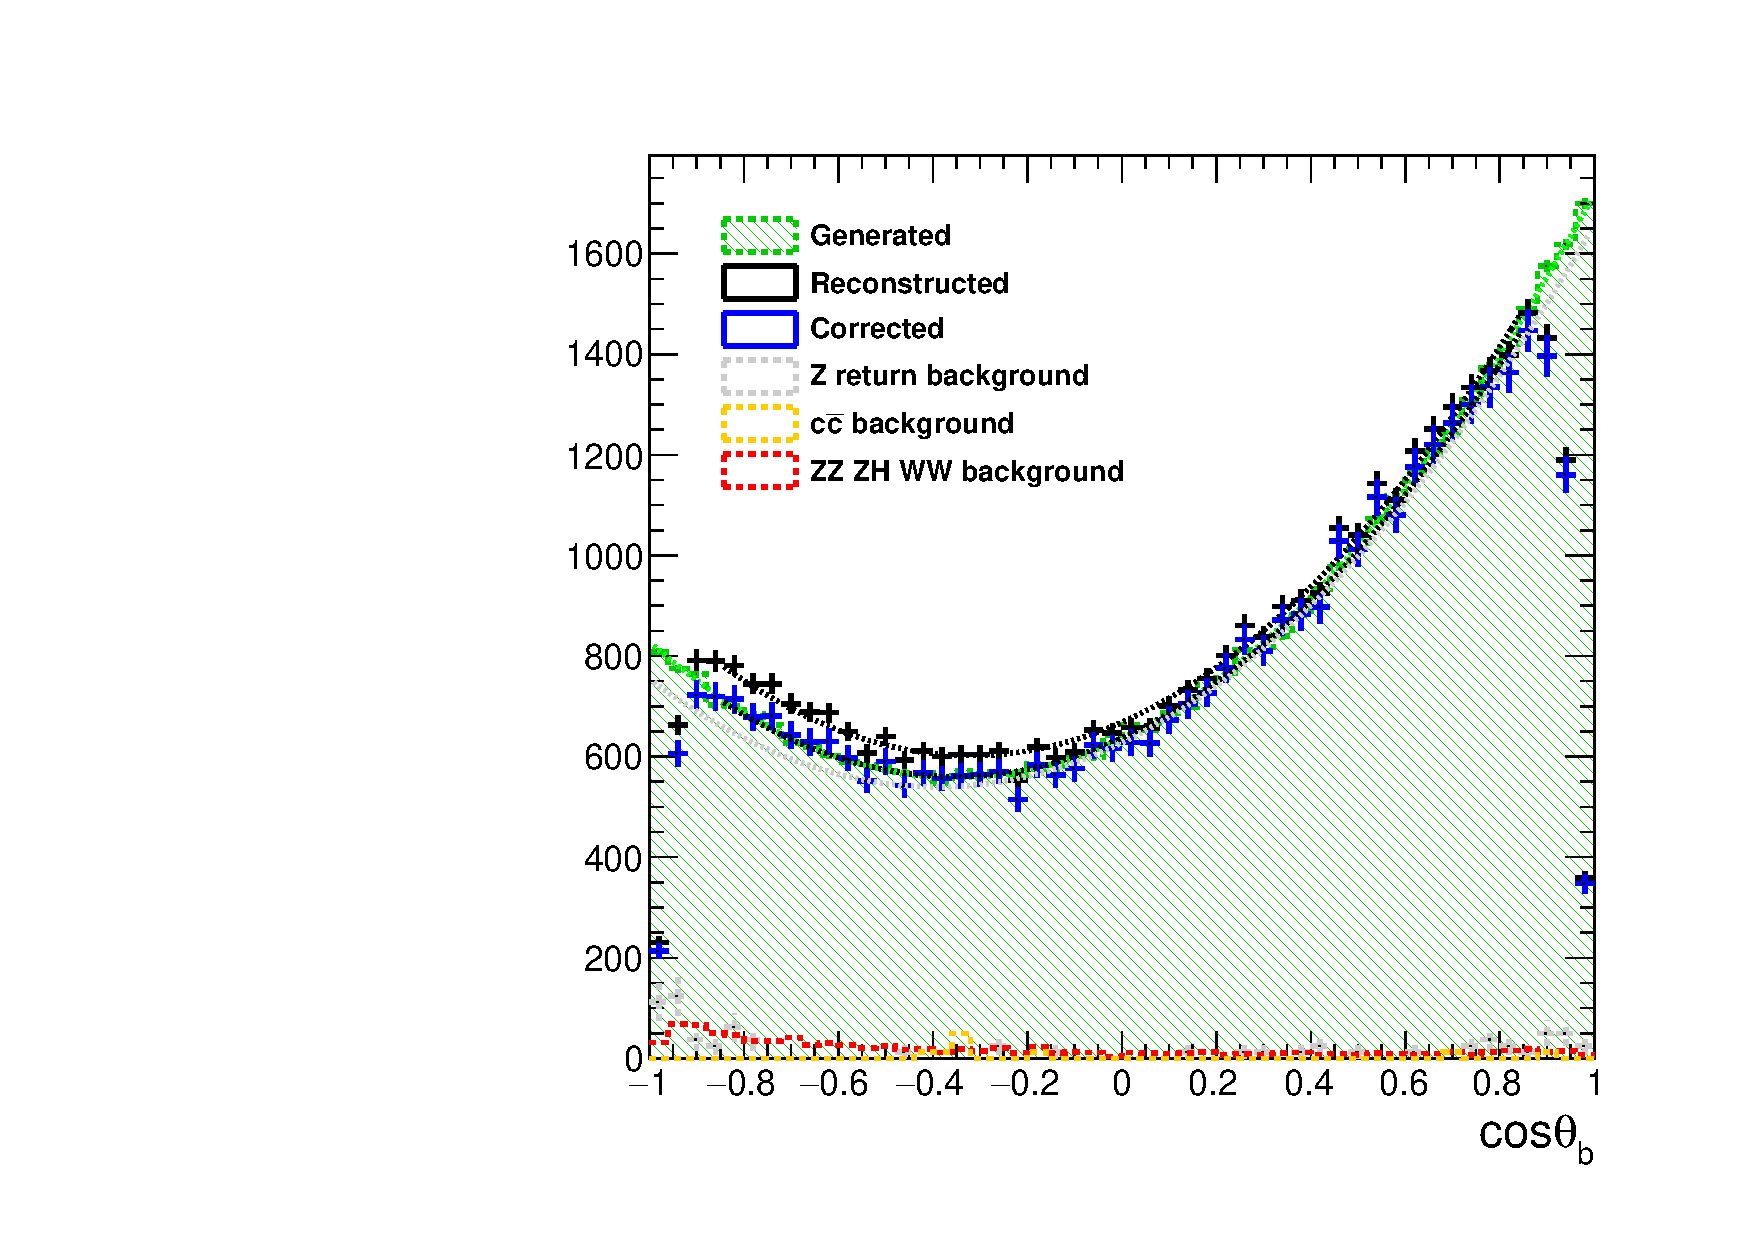
\includegraphics[width=0.49\linewidth]{../ILD/plots/basymmetry-final-right.pdf}
\captionof{figure}{ \sl Generated b-quark polar angle distribution compared to the final reconstructed b-quarks polar angle in left-handed case (a) and right-handed case (b) with overlaid background processes. }
\end{center}\vspace{1cm}

In hac habitasse platea dictumst. Etiam placerat, risus ac.

Adipiscing lectus in magna blandit:

\begin{center}\vspace{1cm}
\begin{tabular}{l l l l}
\toprule
\textbf{Treatments} & \textbf{Response 1} & \textbf{Response 2} \\
\midrule
Treatment 1 & 0.0003262 & 0.562 \\
Treatment 2 & 0.0015681 & 0.910 \\
Treatment 3 & 0.0009271 & 0.296 \\
\bottomrule
\end{tabular}
\captionof{table}{\color{Green} Table caption}
\end{center}\vspace{1cm}

Vivamus sed nibh ac metus tristique tristique a vitae ante. Sed lobortis mi ut arcu fringilla et adipiscing ligula rutrum. Aenean turpis velit, placerat eget tincidunt nec, ornare in nisl. In placerat.

\begin{center}\vspace{1cm}
	\label{fig:LEPILCResult_3}
	\includegraphics[width=0.49\linewidth]{../ILD/plots/lep-result-zoom.pdf}
	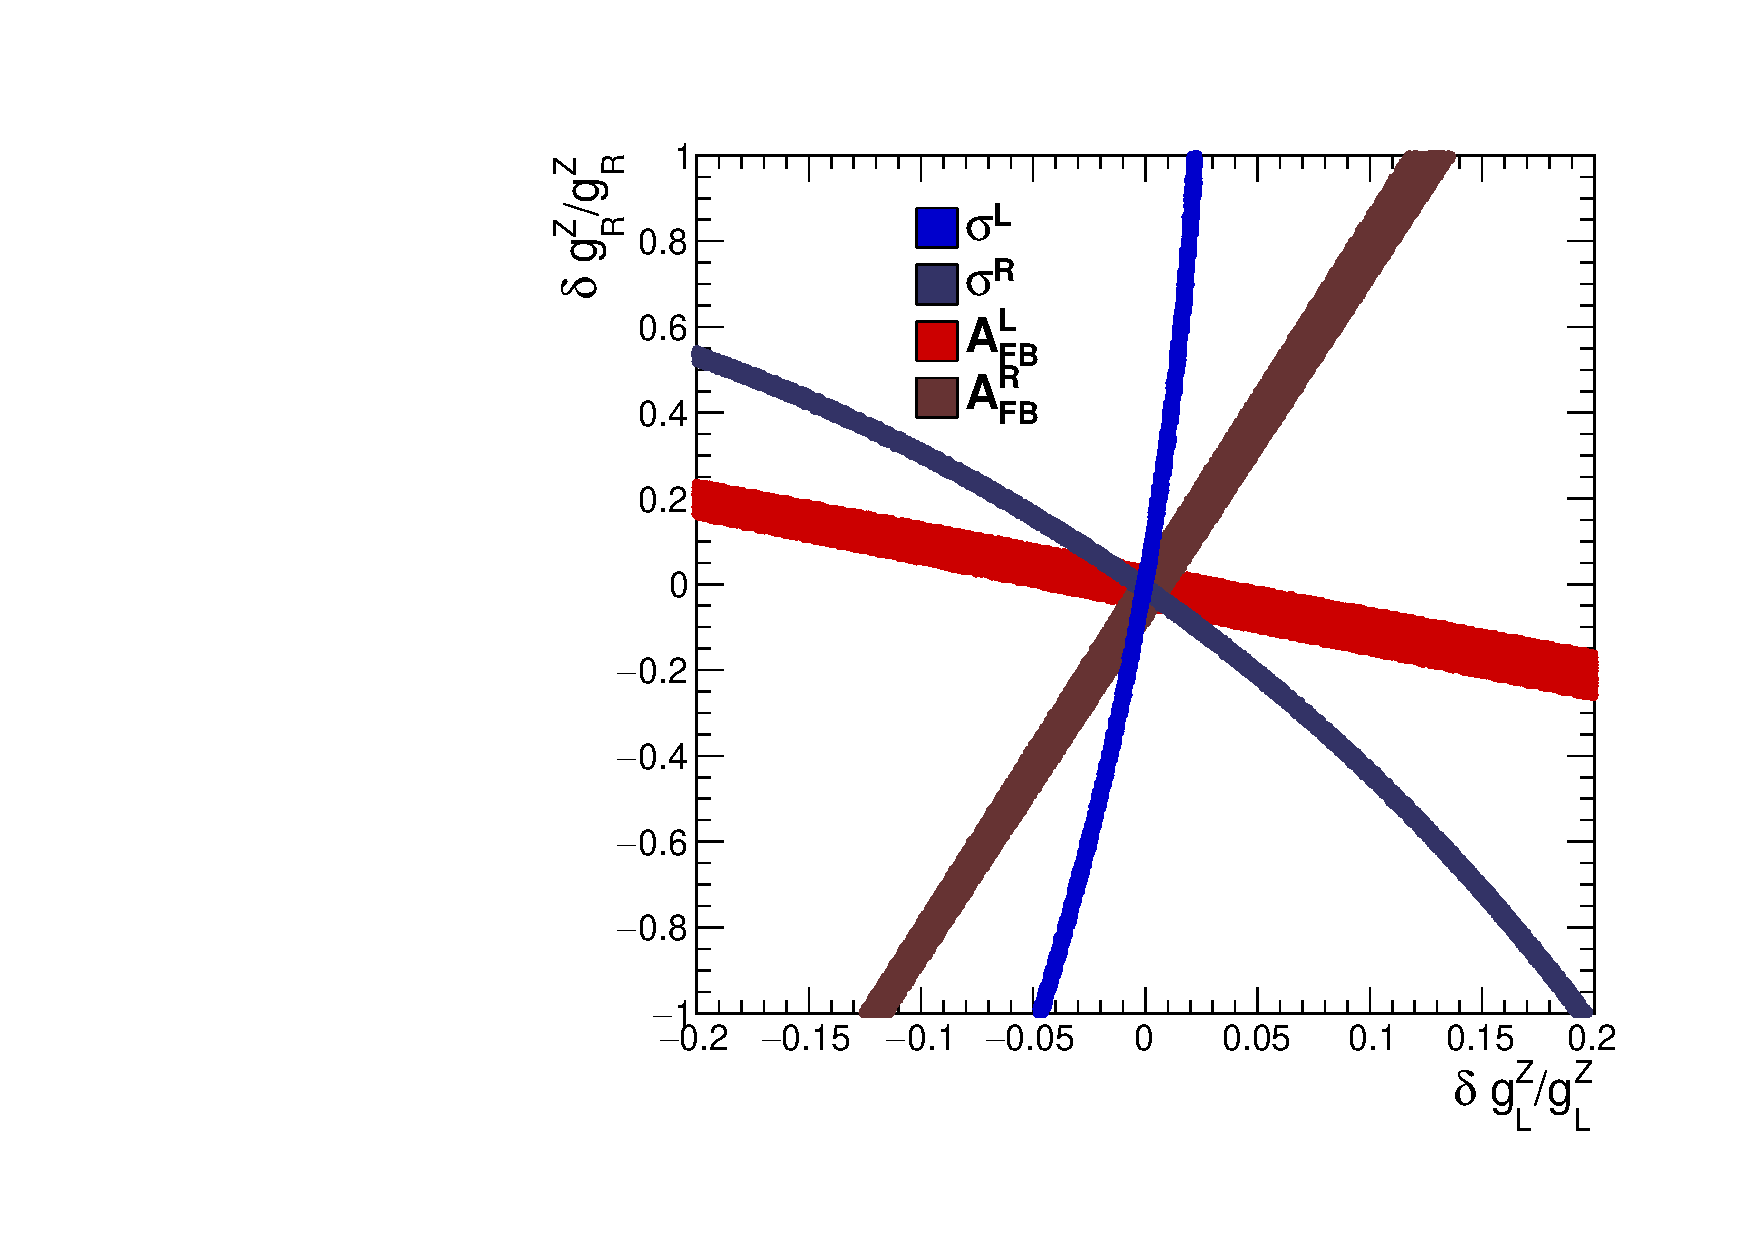
\includegraphics[width=0.49\linewidth]{../ILD/plots/ilc-result.pdf}
	\captionof{figure}{ Tree level $\pm 1\,\sigma$ allowed regions defined by the forward-backward asymmetry and total cross section measurements at LEP (a) and ILC via the differential cross section fit (b). Dashed guidelines show the \sm\ value. The allowed region expected at the ILC is centered at \sm\ values of couplings. }
\end{center}\vspace{1cm}

%----------------------------------------------------------------------------------------
%	CONCLUSIONS
%----------------------------------------------------------------------------------------

\color{SaddleBrown} % SaddleBrown color for the conclusions to make them stand out

\section*{Conclusions}

\begin{itemize}
\item Pellentesque eget orci eros. Fusce ultricies, tellus et pellentesque fringilla, ante massa luctus libero, quis tristique purus urna nec nibh. Phasellus fermentum rutrum elementum. Nam quis justo lectus.
\item Vestibulum sem ante, hendrerit a gravida ac, blandit quis magna.
\item Donec sem metus, facilisis at condimentum eget, vehicula ut massa. Morbi consequat, diam sed convallis tincidunt, arcu nunc.
\item Nunc at convallis urna. isus ante. Pellentesque condimentum dui. Etiam sagittis purus non tellus tempor volutpat. Donec et dui non massa tristique adipiscing.
\end{itemize}

\color{DarkSlateGray} % Set the color back to DarkSlateGray for the rest of the content

%----------------------------------------------------------------------------------------
%	FORTHCOMING RESEARCH
%----------------------------------------------------------------------------------------

\section*{Forthcoming Research}

Vivamus molestie, risus tempor vehicula mattis, libero arcu volutpat purus, sed blandit sem nibh eget turpis. Maecenas rutrum dui blandit lorem vulputate gravida. Praesent venenatis mi vel lorem tempor at varius diam sagittis. Nam eu leo id turpis interdum luctus a sed augue. Nam tellus.

 %----------------------------------------------------------------------------------------
%	REFERENCES
%----------------------------------------------------------------------------------------

\nocite{*} % Print all references regardless of whether they were cited in the poster or not
\bibliographystyle{plain} % Plain referencing style
\bibliography{sample} % Use the example bibliography file sample.bib

%----------------------------------------------------------------------------------------
%	ACKNOWLEDGEMENTS
%----------------------------------------------------------------------------------------

\section*{Acknowledgements}

Etiam fermentum, arcu ut gravida fringilla, dolor arcu laoreet justo, ut imperdiet urna arcu a arcu. Donec nec ante a dui tempus consectetur. Cras nisi turpis, dapibus sit amet mattis sed, laoreet.

%----------------------------------------------------------------------------------------

\end{multicols}
\end{document}